\documentclass[a4paper,norsk,11pt,twoside]{article}
\usepackage[utf8]{inputenc}
\usepackage[T1]{fontenc}
\usepackage[norsk]{babel}
\usepackage{epsfig}
\usepackage{graphicx}
\usepackage{amsmath}
\usepackage{pstricks}
\usepackage{subfigure}
\usepackage{bm}
\usepackage{booktabs}       % Pakke for pene tabeller
                            % http://ctan.uib.no/macros/latex/contrib/booktabs/booktabs.pdf

\usepackage[most]{tcolorbox}

\tcbset{
    frame code={}
    center title,
    left=0pt,
    right=0pt,
    top=0pt,
    bottom=0pt,
    colback=gray!70,
    colframe=white,
    width=\dimexpr\textwidth\relax,
    enlarge left by=0mm,
    boxsep=5pt,
    arc=0pt,outer arc=0pt,
    } 

\date{18.09.2016}
\title{MAT1120 Oblig 1}
\author{Daniel Heinesen, daniehei}

\begin{document}
\maketitle
\newpage

\textbf{Oppgave 1:}

For å finne linkmatrisen ser vi at det går en link fra dokument 1 til 2, 3 og 4. Vi får da en ener i rad 2,3 og 4 i kolonne. Linken fra dokument 2 til 3 og 4 utgjør på samme måte kolonne 2. Linken fra dokument 3 til 1 utgjør kolonne 3, og linkene fra dokument 4 til 1 og 3 utgjør kolonne 4. Siden ingen av dokumentene er linket til seg selv er diagonalen 0. Vi får da matrisen:

$$
\begin{pmatrix}
0 & 0 & 1 & 1\\
1 & 0 & 0 & 0\\
1 & 1 & 0 & 1\\
1 & 1 & 0 & 0\\
\end{pmatrix}
$$

Men for at dette skal være en stokastisk matrise må summen av elementene i kolonnen være lik 1. Vi tar derfor å dele elementene i kolonnen på summen av elementene. Vi får da den stokastiske linkmatrisen:


$$
\begin{pmatrix}
0 & 0 & 1 & 1/2\\
1/3 & 0 & 0 & 0\\
1/3 & 1/2 & 0 & 1/2\\
1/3 & 1/2 & 0 & 0\\
\end{pmatrix}
$$

For å finne den unike scorevektoren vet vi at vi må løse

$$
\textbf{A}\textbf{x} = \textbf{x}
$$
$$
\Rightarrow (\textbf{A} - \textbf{I})\textbf{x} = 0
$$

Vi må altså finne nullrommet til $\textbf{A} - \textbf{I}$. Vi gjør dette ved å radredusere $\textbf{A} - \textbf{I}$:

$$
(\textbf{A} - \textbf{I})
=\begin{pmatrix}
-1 & 0 & 1 & 1/2\\
1/3 & -1 & 0 & 0\\
1/3 & 1/2 & -1 & 1/2\\
1/3 & 1/2 & 0 & -1\\
\end{pmatrix}
$$

$$
\sim \begin{pmatrix}
1 & 0 & 0 & -2\\
0 & 1 & 0 & -2/3\\
0 & 0 & 1 & -3/2\\
0 & 0 & 0 & 0\\
\end{pmatrix}
$$

Dette gir oss at:

$$
x_1 = 2x_4
$$
$$
x_2 = \frac{2}{3}x_4
$$
$$
x_3 = \frac{3}{2}x_4
$$

Og siden det bare er 0'er, som betyrn at $x_4$ er en fri variabel. Setter vi $x_4 = 6$ Dette betyr

$$
Nul(\textbf{A} -\textbf{I}) = span\{ \begin{bmatrix}
12 \\ 4 \\ 9 \\ 6
\end{bmatrix} \}
$$

Alt vi trenger å gjøre nå er å normalisere basisen til nullrommet, og vi har scorevektoren. Summen av elementene i vektoren er $31$. Så den unike scorevektoren er:

$$
\frac{1}{31} \begin{bmatrix}
12 \\ 4 \\ 9 \\ 6
\end{bmatrix}
$$\\


\textbf{Oppgave 2:}

Bruker vi samme metode som over finner vi at linkmatrisen for system 2 er:

$$
\begin{pmatrix}
0 & 1 & 0 & 0 & 0\\
1 & 0 & 0 & 0 & 0\\
0 & 0 & 0 & 1 & 1/2\\
0 & 0 & 1 & 0 & 1/2\\
0 & 0 & 0 & 0 & 0\\
\end{pmatrix}
$$\\

Vi kan allerde her se at vi kommer til å få problemer, siden 1 og 2, og 3 og 4 bare sender frem og tilbake til hverandre noe som betyr at vi ikke kommer til å oppnå noe likevekt mellom dem. Men la oss bevise det matematisk. Vi regner derfor ut $Nul(\textbf{A}-\textbf{I})$:

$$
(\textbf{A}-\textbf{I}) = 
\begin{pmatrix}
-1 & 1 & 0 & 0 & 0\\
1 & -1 & 0 & 0 & 0\\
0 & 0 & -1 & 1 & 1/2\\
0 & 0 & 1 & -1 & 1/2\\
0 & 0 & 0 & 0 & -1\\
\end{pmatrix}
$$
$$
\sim
\begin{pmatrix}
1 & -1 & 0 & 0 & 0\\
0 & 0 & 1 & -1 & 0\\
0 & 0 & 0 & 0 & 1\\
0 & 0 & 0 & 0 & 0\\
0 & 0 & 0 & 0 & 0\\
\end{pmatrix}
$$

Vi setter så opp variablene:

$$
x_1 = x_2
$$
$$
x_3 = x_4
$$
$$
x_5 = 0
$$

Vi har er 2 rader med bare 0'er, som betyr at vi har 2 frie variabler, $x_2$ og $x_4$.

$$
Nul(\textbf{A} -\textbf{I}) = span\{ \begin{bmatrix}
1 \\ 1 \\ 0 \\ 0 \\ 0
\end{bmatrix},
\begin{bmatrix}
0 \\ 0 \\ 1 \\ 1 \\ 0
\end{bmatrix} \}
$$

Siden vi har 2 basiser er det \underline{ikke} mulig å finne en unik scorevektor, som vi antok fra linkmatrisen.\\

\textbf{Oppgave 3):}

Begge matrisen i oppgavene over er stokastiske, siden vi sikret oss om at summen av elementene i kolonnene var 1.\\

For å være regulære må matrisene ha en potens $k$ hvor alle elementene i $A^{k}$ er positive, da vil, for alle potenser $m>k$ $A^{m}$ også bare ha positive elementer. Matrisen vil da ha en unik scorevektor (teorem 18).\\

Matrisen i oppgave 1 har 0-elementer, men sjekker man på matlab finner man at $A^{6}$ har bare positive elementer, og det finnes en unik scorevektor, hvilket vi vet siden vi allerde har funnet den. Denne er derfor regulær.\\

For matrisen i oppgave 2 vet vi allede at det ikke finnes en unik scorevektor, så den kan per teorem 18 ikke være regulær.\\

\textbf{Oppgave 4):}

$$
\textbf{M} = (1-m)\textbf{A} - m\textbf{S}
$$

For å finne om $M$ er stokatisk kan vi summere en virkårlig kolonne, og ser om det blir 1. Kolonnen er:

$$
\textbf{m}_i =
\begin{bmatrix}
(1-m)a_{1i} + m/n\\ \vdots \\ (1-m)a_{ji} + m/n
\end{bmatrix}
$$

Summen av elementene blir:

$$
\sum_j m_{ji} =  (1-m)(\underbrace{a_{1i} + \ldots + a_{ji}}_{=1}) + n\frac{m}{n}
$$
$$
= (1-m) + m = 1
$$

M er derfor stokastisk så lenge \textbf{A} er stokastisk.\\

For at M skal være regulær må elementene være positive. Vi vet at alle elementene i \textbf{A} er $\geq 0$, derfor vil også $(1-m)\textbf{A}$ også være det. $m\textbf{S} = m/n > 0$. Dette betyr at $(1-m)\textbf{A} + m\textbf{S}$ bare har positive elementer. Siden matriseprodukten er dotproduktet av rader og kolonner, hvor alle elementene er positive tall, vil også produktet bare ha positive elementer. Derfor vil $\textbf{M}^{k}$ for $k>0$ bare ha strengt positive elementer, og \textbf{M} er regulær.\\

\textbf{Oppgave 5):}

For linkmatrisen \textbf{A} i oppgave 1, får vi, med $m = 0.15$:

$$
M = 
\begin{pmatrix}
0.03 & 0.88 & 0.03 & 0.03 & 0.03\\
0.88 & 0.03 & 0.03 & 0.03 & 0.03\\
0.03 & 0.03 & 0.03 & 0.88 & 0.455\\
0.03 & 0.03 & 0.88 & 0.03 & 0.455\\
0.03 & 0.03 & 0.03 & 0.03 & 0.03\\
\end{pmatrix}
$$

Ved bruk av matlab finner vi at:

$$
Nul(\textbf{M} - \textbf{I}) = span\{ \begin{bmatrix}
-0.405429 \\ -0.405429 \\ -0.577736 \\ -0.577736 \\ -0.060814
\end{bmatrix} \}
$$

Normaliserer vi basisen finenr vi scorevektoren for \textbf{M}

$$
\begin{bmatrix}
0.2 \\ 0.2 \\ 0.285 \\ 0.285 \\ 0.03
\end{bmatrix}
$$\\

\textbf{Oppgave 6):}

Det denne funksjonen gjør er at den lager en matrise med 0'ere og 1'ere spredd tilfeldig i matrisen, deretter sjekker den om det er noen kolonner som bare inneholder 0'ere, og om det er tilfelle blir en 1'er lagt til. Elementene i diagonalen blir satt til 0. Tilslutt normaliseres kolonnene. \\

Siden alle kolonnene nå bare har positive elementer og summen av elementene er 1, så har vi en stokastisk matrise. Men vi ville ikke at noen av dokumentene skal linke til seg selv, men siden diagonalen bare inneholder 0'er, vil dette være tilfellet. Dette betyrn at alle kravene for en linkmatrise er oppfylt.\\

\textbf{Oppgave 7):}

Jeg får den tilfeldige linkmatrisen:

$$
\begin{pmatrix}
0 & 0 & 1/3 & 1/2 & 1/3 \\
0 & 0 & 1/3 & 1/2 & 0 \\
0 & 0 & 0 & 0 & 1/3 \\
0 & 0 & 1/3 & 0 & 1/3 \\
1 & 1 & 0 & 0 & 0
\end{pmatrix}
$$ 

Linkdiagrammet blir:

\begin{figure}[hbt]
\begin{center}
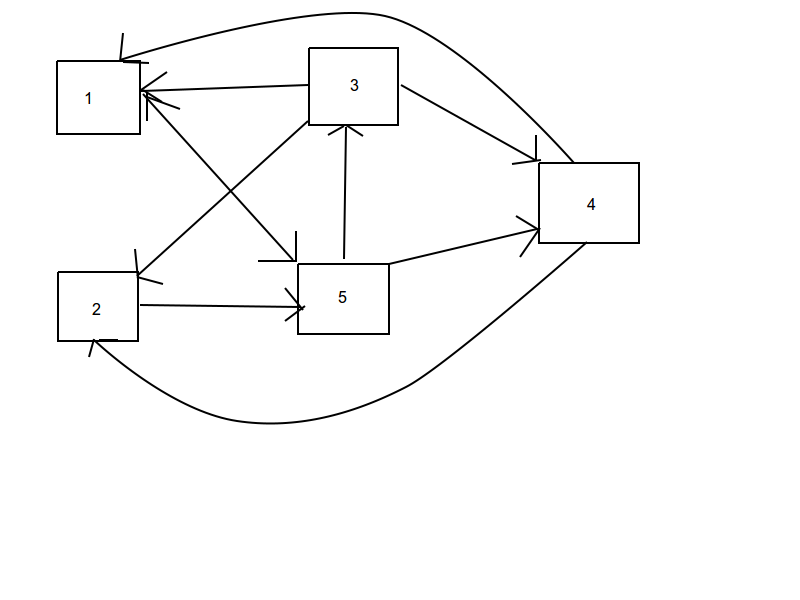
\includegraphics[width=70mm]{linkdiagram.png}
\caption{Et litt forvirrende diagram}\label{fig:finfigur}
\end{center}
\end{figure} 


\textbf{Oppgave 10):}

Som i oppgave 1 er

$$
A = 
\begin{pmatrix}
0 & 0 & 1 & 1/2\\
1/3 & 0 & 0 & 0\\
1/3 & 1/2 & 0 & 1/2\\
1/3 & 1/2 & 0 & 0\\
\end{pmatrix}
$$


Vi kan få scorevektoren til $\textbf{M}(\textbf{A})$ ved både den nøyaktige utregningen og tilnærmingen. Vi kan forvente at for små $\delta$ skal disse være ganske like.\\

Ved bruk av $ranking$-funksjonen får jeg at scorevektoren for $M$ er

$$
\textbf{x} = \begin{bmatrix}
0.36815 \\ 0.14181 \\ 0.28796 \\ 0.20208 
\end{bmatrix}
$$

Ved bruk av $rankingapprox$ med $\delta = 0.005$ får vi

$$
\textbf{x} = \begin{bmatrix}
0.36639 \\ 0.14224 \\ 0.28840 \\ 0.20297
\end{bmatrix}
$$

Vi kan se at disse 2 vektorene nesten er like, som vi forventer av funksjonene. Senker vi $\delta$ litt vil de komme nærmere hverandre, og ved $\delta = 0.0005$ vil de allerde være like hverandre ned til den 5 desimalspresisjonen jeg har brukt her.



\end{document}